\documentclass[11pt]{exam}		%Doc : https://mirrors.ircam.fr/pub/CTAN/macros/latex/contrib/exam/examdoc.pdf

% \printanswers					%Comment this line to hide the answers 

\pointpoints{point}{points}
\addpoints

%----------------------------------------------------------------------------------------
%	PACKAGES AND OTHER DOCUMENT CONFIGURATIONS
%----------------------------------------------------------------------------------------

\usepackage{lastpage} % Required to determine the last page number for the footer

\usepackage[utf8]{inputenc}
\usepackage[T1]{fontenc}
\usepackage[french]{babel}      %Originally for french document, change to english or relevant language

\usepackage{amsmath,amssymb}
\usepackage{multicol}
\usepackage[dvipsnames,svgnames]{xcolor}
\usepackage{tikz}
\usetikzlibrary{fadings}
\usetikzlibrary{calc}

\usepackage{tkz-tab}
\usepackage{pgfplots}
\pgfplotsset{compat=1.17}


\usepackage{multido} % required for answerbox
\usepackage[most]{tcolorbox} % Required for boxes that split across pages

\usepackage{atbegshi}
\usepackage{etoolbox}
\usepackage{transparent}
\usepackage{eso-pic}

%----------------------------------------------------------------------------------------
%	MARGINS
%----------------------------------------------------------------------------------------

\usepackage{geometry} % Required for adjusting page dimensions and margins

\geometry{
	paper=a4paper, % Change to letterpaper for US letter
	top=1.5cm, % Top margin
	bottom=2.5cm, % Bottom margin
	left= 1cm, % Left margin
	right=1cm, % Right margin
	headheight=14pt, % Header height
	footskip=1.4cm, % Space from the bottom margin to the baseline of the footer
	headsep=14pt, % Space from the top margin to the baseline of the header
	%showframe, % Uncomment to show how the type block is set on the page
}

%----------------------------------------------------------------------------------------
%	FONT
%----------------------------------------------------------------------------------------
\usepackage{fontspec}
\usepackage{unicode-math}
\usepackage[utf8]{inputenc} % Required for inputting international characters
\usepackage[T1]{fontenc} % Output font encoding for international characters

% \usepackage[sfdefault,light]{roboto} % Use the Roboto font
\setmainfont[Ligatures=TeX]{Caladea}

%----------------------------------------------------------------------------------------
%	HEADERS AND FOOTERS
%----------------------------------------------------------------------------------------


%Format Header and footer
\pagestyle{headandfoot}
\header{Physique Chimie}{\Large\textbf{Chapitre 1}}{
	\footnotesize  
	Classe : \ldots\ldots\ldots\ldots\ldots\ldots
	\\ Nom et prénom: \ldots\ldots\ldots\ldots\ldots\ldots\ldots\ldots\ldots\ldots\ldots\ldots\ldots\ldots\ldots\ldots\ldots\ldots 
}
\headrule
\footrule
\setlength{\columnsep}{0.25cm}
\setlength{\columnseprule}{1pt}
\footer{}{ Page \thepage \hphantom s sur \pageref{LastPage} }{}
% \extrafootheight{-2cm}

\pagestyle{plain}
% Change section command behaviour
\usepackage{titlesec}
% \titleformat{\section}[frame]{\Huge\bfseries\filright}{}{2mm}{\centering Devoir surveillé: }

\titleformat
{\section} % Section type being modified
[frame] % Shape type, can be: hang, block, display, runin, leftmargin, rightmargin, drop, wrap, frame
{\Huge\bfseries\filright} % Format of the whole section
{\thesection} % Format of the section label
{6pt} % Space between the title and label
{\centering Devoir surveillé: } % Code before the label


\usepackage{titling} % Allows custom title configuration



\pretitle{
	\vspace{200pt} % Move the entire title section up
}


% \titlespacing{\section}{0pt}{0.5\baselineskip}{0.5\baselineskip} % Spacing around section titles, the order is: left, before and after



% Add a watermark if answers are shown
\ifprintanswers
\usepackage{draftwatermark}
\SetWatermarkColor{red!30}
\SetWatermarkScale{1.1}
\SetWatermarkText{Correction}     %Watermark text
\fi



% contains the answer to a question or a box where the student can reply
% #1 number of lines to reply
% #2 answer to the question, centered
\newcommand{\answerbox}[2]{
	\ifprintanswers
		\begin{center}
			\color{DarkRed}
			\textbf{\textit{#2}}
		\end{center}

	\else
	\begin{tcolorbox}[breakable, enhanced]
		\vspace{7pt}
		\multido{}{#1}{\noindent\makebox[\linewidth]{\dotfill}\endgraf\vspace{5pt}}% ... dotted lines ...
	\end{tcolorbox}
	\fi
}

\renewcommand*\half{.5}

% \qformat{\textbf{\large Question \thequestion\hfill}  (\thepoints)}


\AtBeginShipout{
\ifnumodd{\thepage}{

\AddToShipoutPictureBG*{
    % \includegraphics[]{example-grid-100x100bp}}
    % \transparent{0.4}
    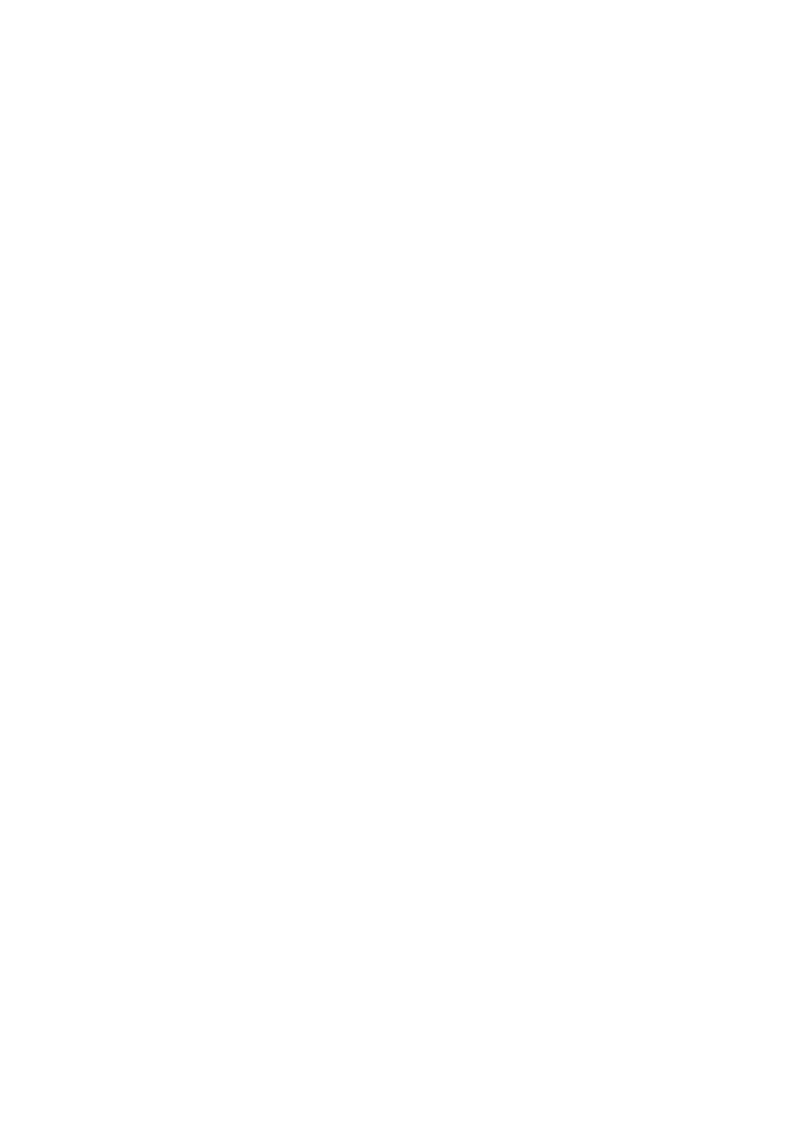
\includegraphics[]{bg1.png}
    }
}{

\AddToShipoutPictureBG*{
    % \includegraphics[]{example-grid-100x100bp}}
    % \transparent{0.4}
    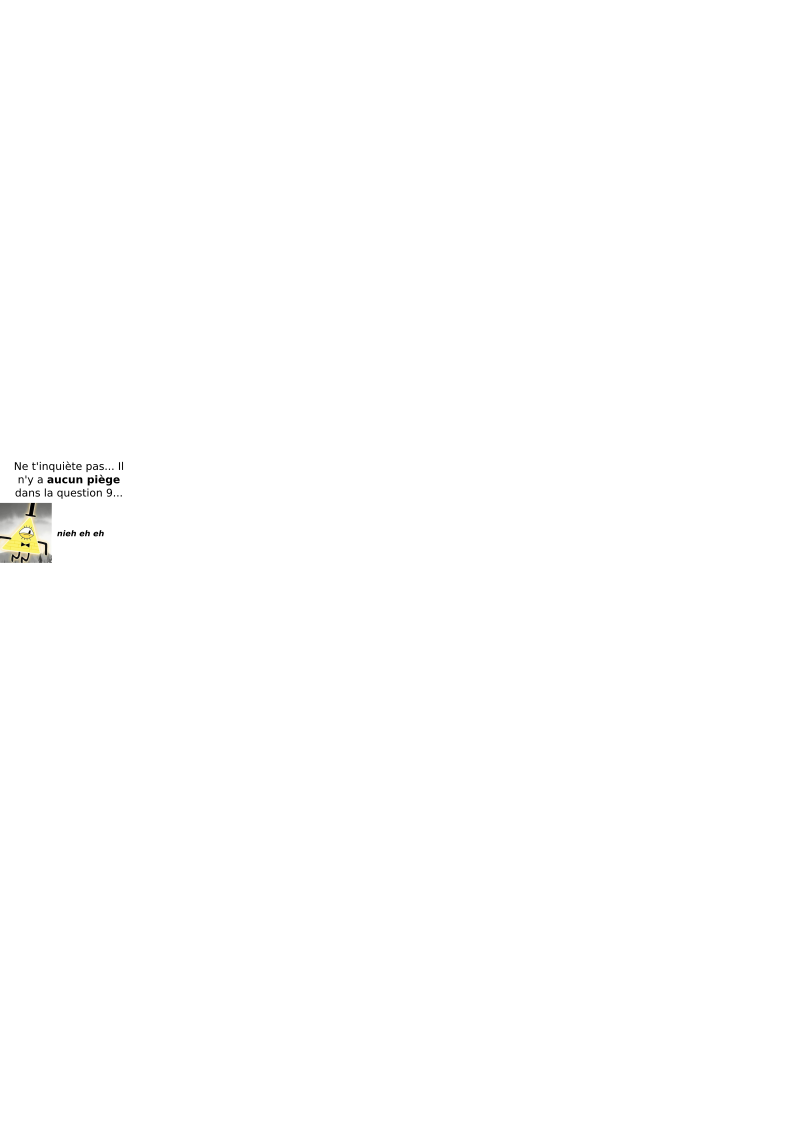
\includegraphics[]{bg2.png}
    }
}

}

\AddToShipoutPictureBG*{
    % \includegraphics[]{example-grid-100x100bp}}
    % \transparent{0.4}
    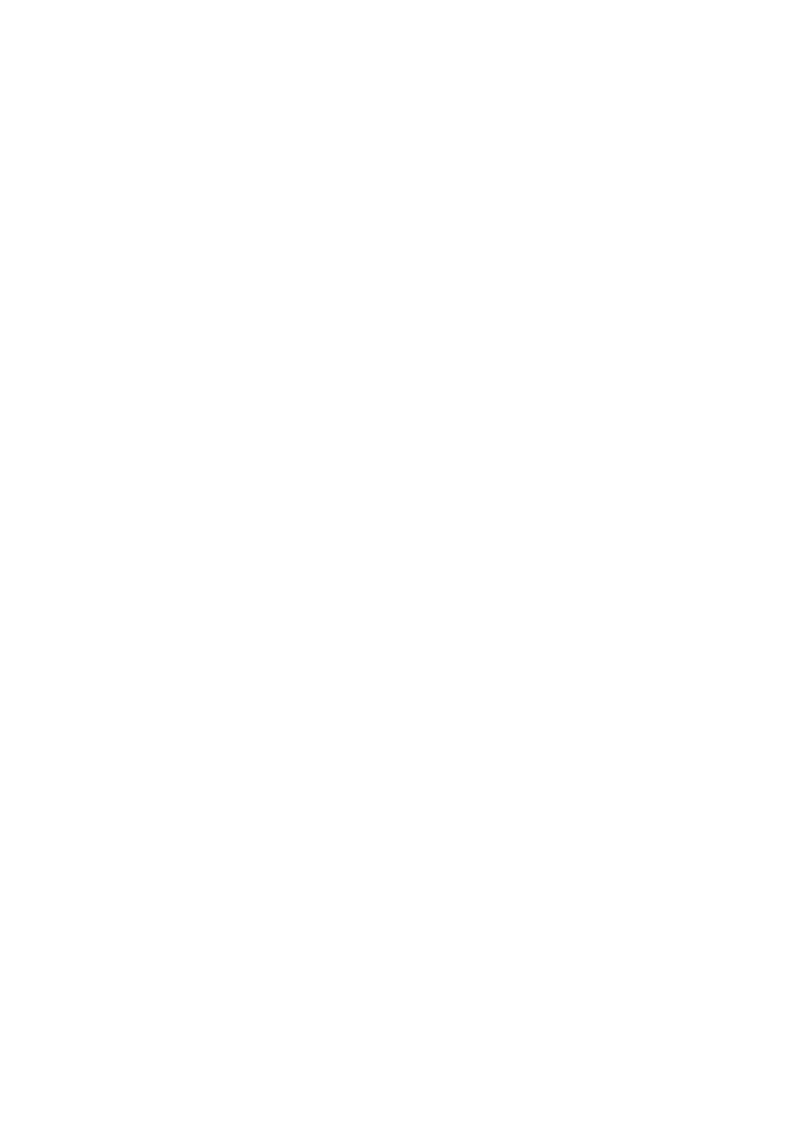
\includegraphics[]{bg1.png}
    }
\usepackage{blindtext, subfig}
\usepackage{dblfloatfix} % fix for bottom-placement of figure

%----------------------------------------------------------------------------------------
%	REQUIRED
%----------------------------------------------------------------------------------------
\newcommand{\Titre}{Électricité (le retour)} % 
\newcommand{\ConsignesGenerales}{
	
	\begin{itemize}
		\item Noter nom et prénom et classe en haut à gauche de la page.
		\item Répondre aux questions sur les pointillés.
		\item Répondre aux questions par des phrases.
		\item Essayer de répondre à toutes les questions.
		\item Ne pas perdre trop de temps si on ne sait pas/comprends 
		pas et passer à la suite pour avoir un maximum de points! 
		% \item Ne pas se décourager :)
		\vspace{-5pt}
	\end{itemize}}

\title{\Titre}
\begin{document}
\thispagestyle{headandfoot}

\section{\Titre} % peut faire une partie d'un gros examen

\headrule
\footrule
\setlength{\columnsep}{0.25cm}
\setlength{\columnseprule}{1pt}



\begin{center}
	\begin{tcolorbox}[
		title=Consignes,
		sidebyside,
		colback=red!5!white,
		colframe=red!75!black,
		colbacktitle=yellow!30!red!50!white,
		coltitle=red!25!black,
		fonttitle=\bfseries,
		subtitle style={boxrule=0.4pt,
		colback=yellow!50!red!25!white} ]
		\ConsignesGenerales

		\tcblower

		% \tcbincludegraphics[width=0.2\columnwidth]{logo.png}
		\tcbincludegraphics[height=3.5cm, size=tight, colframe=red, boxrule=1pt, arc=10pt, auto outer arc, clip upper]{logo.png}
		
		% \tcbsubtitle{Second subtitle}
		% Further text.
		\end{tcolorbox}
\end{center}

%----------------------------------------------------------------------------------------
%	Partie Cours
%----------------------------------------------------------------------------------------
{\huge Partie cours}
	\begin{questions}
		\question[1] 
		Que signifie l'acronyme D.E.L. ? : \dotfill

		\question[1] 
		Le sens du courant a t-il une 
		influence sur le fonctionnement 
		de la lampe ? : \dotfill

		\question[1\half] 
		Un moteur est-il un générateur ou un récepteur? 
		\textbf{Justifier}.
		\answerbox{2}{
			Le moteur est un récepteur, 
			sans électricité il ne fonctionne pas.
		}

		\question[1\half] 
		\textbf{Expliquer} quelle influence le sens du 
		courant a t-il une sur le fonctionnement d'un moteur? 
		\answerbox{2}{
			Le moteur tourne dans un 
			sens différent si le sens du courant est différent.
		}

		\question[2] 
		\textbf{Expliquer} le principe de fonctionnement
										\footnote{
											C'est à dire, ce qu'il se passe quand on le fait fonctionner.
											}
			d'un moteur électrique.
		\answerbox{2}{
			Le moteur est un utilise de l'électricité pour
			se mettre en mouvement.
		}

		\question[2]
		\textbf{Expliquer} le principe de fonctionnement
		d'un interrupteur.
		\answerbox{2}{
			Pour couper le courant d'un circuit, l'interrupteur rompt 
			la boucle de courant.
		}

		\question[2] 
		Dans un circuit électrique contenant un unique générateur,
		\textbf{énoncer} dans quel sens circule 
		le courant.
		\answerbox{2}{
			Le courant circule de la borne positive ”+” à 
			la borne négative ”-”
			à l’extérieur du générateur.
		}

%----------------------------------------------------------------------------------------
%	Partie Application
%----------------------------------------------------------------------------------------


% \vspace{30pt}
\newpage
{\huge Partie application}
	\question[3] Le court circuit :

	\textit{(a) (1 points)} Rappeler la définition du court circuit.
	\footnote{c'est à dire quand est-ce qu'un dipôle est court circuité}.
	\answerbox{2}{
		Un dipôle est court circuité quand ses deux 
		bornes sont directement relié par un matériau conducteur.
		}
	\textit{(b) (2 points)} 
	Pour les schémas suivants, \textbf{indiquer en dessous du schéma} si un dipôle est court circuité et lequel.
	
	\begin{figure*}[hb]
		\centering
		\subfloat[][]{
			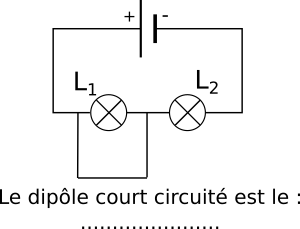
\includegraphics[width=5cm]{short1.png}
			}
			\hspace{180pt}
		\subfloat[][]{
			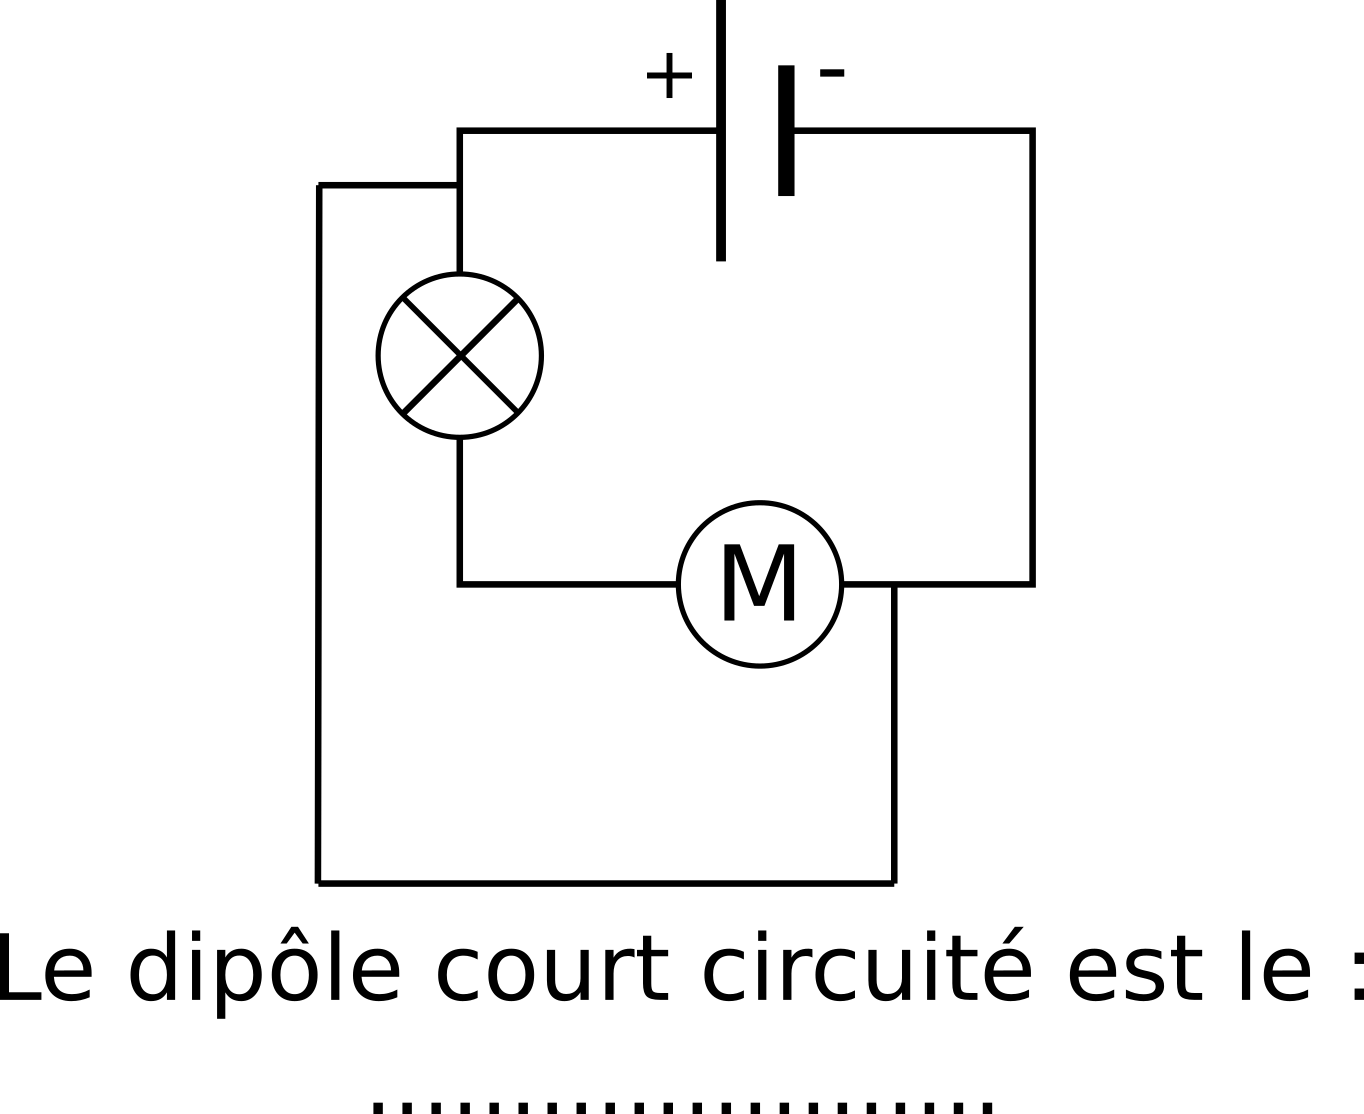
\includegraphics[width=5cm]{short2.png}
		 }
	\end{figure*}
		



	\question[4]
	Pour chacun des schéma suivants, \textbf{indiquer sur le schéma} le sens du courant.

	\begin{figure*}[hb]
		\centering
		\hspace{70pt}
		\subfloat[][]{
			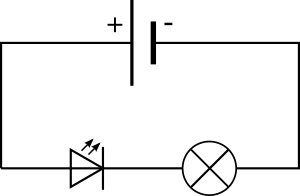
\includegraphics[width=3cm]{sens1.png}
			}
			\hspace{20pt}
		\subfloat[][]{
			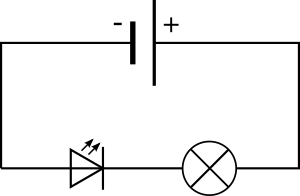
\includegraphics[width=3cm]{sens2.png}
		 }
			\hspace{20pt}
			\subfloat[][]{
			 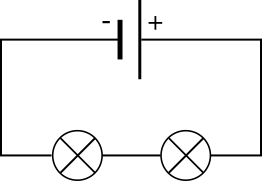
\includegraphics[width=3cm]{sens3.png}
		  }
			\hspace{20pt}
			\subfloat[][]{
			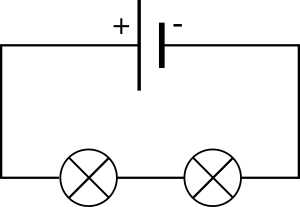
\includegraphics[width=3cm]{sens4.png}
		}
	\end{figure*}
		



	\question[2]
	Pour chacun des schéma suivants, \textbf{indiquer en dessous du schéma} 
	si la DEL est dans le sens passant ou dans le sens bloquant.

	\begin{figure*}[hb]
		\centering
		\subfloat[][]{
			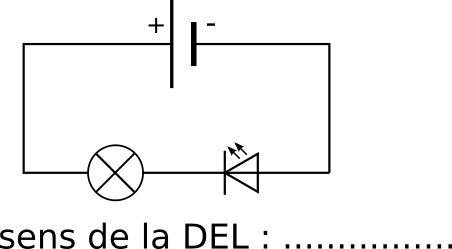
\includegraphics[width=5cm]{del1.png}
			}
			\hspace{180pt}
		\subfloat[][]{
			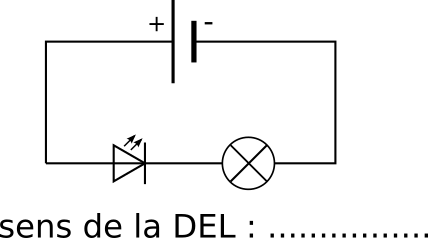
\includegraphics[width=5cm]{del2.png}
		 }
	\end{figure*}
		




\end{questions}


\vfill
\begin{center}
\setlength{\doublerulesep}{0.25in}
\multirowgradetable{1}[questions]
% \vspace{-25pt}
\end{center}


\end{document}